\PassOptionsToPackage{colorlinks=true,linkcolor=blue,urlcolor=blue}{hyperref}



\documentclass[11pt]{article}

%\usepackage[top=1in, bottom=1in, left=1cm, right=1cm]{geometry}
%\usepackage{lipsum}
%\usepackage{background}
%\backgroundsetup{
%  position=current page.east,
%  angle=-90,
%  nodeanchor=east,
%  vshift=-5mm,
%  opacity=1,
%  scale=3,
%  contents=Confidential
%}

\usepackage{amsmath,amssymb,amsthm,bm}   % TeX4ht relies on these
\usepackage{mathtools}            % optional but harmless
\usepackage{rotating}

\usepackage[margin=1cm, paperwidth=8.5in, paperheight=11in]{geometry}
\usepackage[
  hypertexnames=false
]{hyperref}
\usepackage{kotex}
\usepackage{etex}
\usepackage{fullpage}
\usepackage{mathtools}
\usepackage{amsfonts}
\usepackage{graphicx}
\usepackage{amsthm}
\usepackage[utf8]{inputenc}
\usepackage{afterpage}
\usepackage{adjustbox}
\usepackage{placeins}
\usepackage{fixltx2e}
\usepackage{supertabular} 
\usepackage{titlesec}
\usepackage{array}
\usepackage{tabularx}
\usepackage{color}
\usepackage{algorithm}
\usepackage{algpseudocode}
\usepackage{subcaption}
\usepackage{hyperref}
\usepackage{pgfplots}
\usepackage{relsize}
\let\labelindent\relax
\usepackage{enumitem}
\usepackage{fancyhdr}
\usepackage{alltt}
\usepackage{soul}
\usepackage{fancyvrb}
\usepackage{xcolor}
%\usepackage[english,greek]{babel}
%\usepackage{ucs} 
%\usepackage[utf8x]{inputenc}
%\usepackage[usenames,dvipsnames]{xcolor}
%\usepackage{tikz}
%\usepackage{tkz-tab}
%\usepackage{caption}
%\usepackage{latexsym}
%\usepackage{amssymb}
\usepackage[margin=0.1cm]{subcaption}
\usepackage{multicol}
\usepackage{refcount}

\usepackage{breakurl} % Break URL
\usepackage{multirow}
\usepackage[most]{tcolorbox}
%\usepackage[breakable,skins]{tcolorbox}

\tcbset{breakable}
\usepackage{esvect}
\usepackage{hyperref}
\usepackage{mathdots}
\usepackage{pifont} 
\usepackage{booktabs}
\usepackage{arydshln}
\usepackage{xcolor}
\def\UrlBreaks{\do\/\do-}
\usepackage{mathtools}  
\usepackage{array}
\usepackage{hyperref}
\usepackage{hyperref}
\usepackage{mathtools, nccmath}
%\usepackage[style=numeric,sorting=none]{biblatex}

\usepackage{titling}
\renewcommand\maketitlehooka{\null\mbox{}\vfill}
\renewcommand\maketitlehookd{\vfill\null}

\DeclarePairedDelimiter{\nint}\lfloor\rceil

\DeclarePairedDelimiter{\abs}\lvert\rvert
\usepackage{tocloft}
\usepackage{pdflscape}
\usepackage[all=normal, floats, bibnotes, wordspacing, charwidths, indent]{savetrees}
\makeatletter%
\captionsetup{belowskip=0pt}

\usepackage{enumitem}
\setlist{nolistsep}
%\setlist[itemize]{leftmargin=0.1}
\setlist[itemize]{leftmargin=*}
\setlist[enumerate]{leftmargin=*}

% align figures to the top margin
\makeatletter
\setlength{\@fptop}{0pt}

\newcommand\bunderline{}% check for being undefined
\DeclareRobustCommand\bunderline[1]{\mathord{\mathpalette\b@underline{#1}}}
\newcommand{\b@underline}[2]{%
  \sbox\z@{$\m@th#1\underline{#2}$}%
  \raisebox{-\dp\z@}{\scalebox{.5}[.25]{$\m@th#1[$}}%
  \copy\z@
  \raisebox{-\dp\z@}{\scalebox{.5}[.25]{$\m@th#1]$}}%
}


\makeatother

%\renewcommand{\figureautorefname}{foo}
%\renewcommand{\tableautorefname}{bar}

%\usepackage[all=normal, floats, bibnotes, wordspacing, charwidths, indent, lists]

%\captionsetup{belowskip=0pt}

\usepackage{graphicx}
\def\rotatecharone#1{\rotatebox[origin=c]{180}{#1}}

\def\rotatechartwo#1{\reflectbox{#1}}
\usepackage{hyperref}
\skip\footins 0.5\baselineskip %8.1pt plus 4pt minus 2pt
\floatsep 0.5\baselineskip
\textfloatsep 0.5\baselineskip
\intextsep 0.5\baselineskip 
\dbltextfloatsep 0.5\baselineskip  
\dblfloatsep 0.5\baselineskip 

%\raggedbottom

\belowcaptionskip 0pt

\everypar{\looseness=-1 }

\setlength{\abovecaptionskip}{0pt} % 

\newenvironment{myproof}[1][\proofname]{%
  \begin{proof}[#1]$ $\par\nobreak\ignorespaces
}{%
  \end{proof}
}
\makeatletter
\renewcommand{\sectionautorefname}{\S\@gobble}
\renewcommand{\subsectionautorefname}{\S\@gobble}
\renewcommand{\subsubsectionautorefname}{\S\@gobble}
\renewcommand{\appendixautorefname}{\S\@gobble}
\renewcommand{\appendixautorefname}{\S\@gobble}

\newcommand\mymathcolor[2]{{\color{#1}#2}}

\makeatother
\newcommand{\ignore}[1]{}

% Add additional comma in the math mode
%\DeclareMathSymbol{,}{\mathpunct}{letters}{"2C}
%\newcommand{\comma}{\mathpunct{\mkern\thinmuskip}}
%\mathcode`,=\string"8000
%{\catcode`,=\active \gdef,{\comma}}


\addtolength{\cftsecnumwidth}{15pt}
\addtolength{\cftsubsecnumwidth}{10pt}
\addtolength{\cftsubsubsecnumwidth}{10pt}

\makeatletter%
\usepackage{stackengine,xcolor}
\input pdf-trans
\newbox\qbox
\def\usecolor#1{\csname\string\color@#1\endcsname\space}
\newcommand\bordercolor[1]{\colsplit{1}{#1}}
\newcommand\fillcolor[1]{\colsplit{0}{#1}}
\newcommand\colsplit[2]{\colorlet{tmpcolor}{#2}\edef\tmp{\usecolor{tmpcolor}}%  
  \def\tmpB{}\expandafter\colsplithelp\tmp\relax%
  \ifnum0=#1\relax\edef\fillcol{\tmpB}\else\edef\bordercol{\tmpC}\fi}
\def\colsplithelp#1#2 #3\relax{%
  \edef\tmpB{\tmpB#1#2 }%
  \ifnum `#1>`9\relax\def\tmpC{#3}\else\colsplithelp#3\relax\fi
}
\newcommand\outline[1]{\leavevmode%
  \def\maltext{#1}%
  \setbox\qbox=\hbox{\maltext}%
  \boxgs{Q q 2 Tr \thickness\space w \fillcol\space \bordercol\space}{}%
  \copy\qbox%
}
\newcommand\mathcalbb[2][1]{%
  \stackengine{0pt}{\def\thickness{.55}\outline{$\mathcal{#2}$}}{\kern.1pt\outline{$\mathcal{#2}$}}{O}{l}{F}{F}{L}}
\bordercolor{black}
\fillcolor{white}
\def\thickness{.1}% TO CHANGE THICKNESS OF SHADOW
\usepackage{lmodern}
\usepackage{lipsum}


\makeatletter
\DeclareRobustCommand{\ccong}{\mathrel{\mathpalette\@verequiv\sim}}
\newcommand{\@verequiv}[2]{%
  \lower.5\p@\vbox{
    \lineskiplimit\maxdimen
    \lineskip-.5\p@
    \ialign{%
      $\m@th#1\hfil##\hfil$\crcr
      #2\crcr
      \equiv\crcr
    }%
  }%
}
\renewcommand*\env@matrix[1][c]{\hskip -\arraycolsep
  \let\@ifnextchar\new@ifnextchar
  \array{*\c@MaxMatrixCols #1}}


\newcommand{\hathat}[1]{% 
\begingroup%
  \let\macc@kerna\z@%
  \let\macc@kernb\z@%
  \let\macc@nucleus\@empty%
  \hat{\raisebox{.2ex}{\vphantom{\ensuremath{#1}}}\smash{\hat{#1}}}%
\endgroup%
}

\newcommand{\revise}[1]{{{\textcolor{black}{#1}}}}

\makeatother

% \title{**\vspace*{\fill}**The Beginner's Textbook for Fully Homomorphic Encryption}

% \date{January 1, 2025}

% \author{Ronny Ko**\vspace*{\fill}**}


\begin{document}
\title{\Huge{\textbf{The Beginner's Textbook}}\\ \Huge{\textbf{for Fully Homomorphic Encryption}}}
\author{\textbf{}\\{LG Electronics Inc.}}%\\\texttt{\small{hajoon.ko@lge.com}}}
\date{January 1, 2025}



\begin{titlingpage}
\maketitle
\end{titlingpage}


\clearpage

\section*{Preface}
Fully Homomorphic Encryption (FHE) is a cryptographic scheme that enables computations to be performed directly on encrypted data, as if the data were in plaintext. After all computations are performed on the encrypted data, it can be decrypted to reveal the result. The decrypted value matches the result that would have been obtained if the same computations were applied to the plaintext data.

FHE supports basic operations such as addition and multiplication on encrypted numbers. Using these fundamental operations, more complex computations can be constructed, including subtraction, division, logic gates (e.g., AND, OR, XOR, NAND, MUX), and even advanced mathematical functions such as ReLU, sigmoid, and trigonometric functions (e.g., sin, cos). These functions can be implemented either as exact formulas or as approximations, depending on the trade-off between computational efficiency and accuracy. 

FHE enables privacy-preserving machine learning by allowing a server to process the client’s data in its encrypted form through an ML model. With FHE, the server learns neither the plaintext version of the input features nor the inference results. Only the client, using their secret key, can decrypt and access the results at the end of the service protocol.
FHE can also be applied to confidential blockchain services, ensuring that sensitive data in smart contracts remains encrypted and confidential while maintaining the transparency and integrity of the execution process.
Other applications of FHE include secure outsourcing of data analytics, encrypted database queries, privacy-preserving searches, efficient multi-party computation for digital signatures, and more.

This book is designed to help the reader understand how FHE works from the mathematical level. The book comprises the following four parts: 

$ $

\begin{itemize}
\item \textbf{\autoref{part:basic-math}:~\nameref{part:basic-math}} explains necessary background concepts for FHE, such as Group, Field, Order, Polynomial Ring, Cyclotomic Polynomial, Vectors and Matrices, Chinese Remainder Theorem, Taylor Series, Polynomial Interpolation, and Fast Fourier Transform.

\item \textbf{\autoref{part:pqc}:~\nameref{part:pqc}} explains well-known lattice-based cryptographic schemes, which are LWE, RLWE, GLWE, GLev, and GGSW cryptosystems.

\item \textbf{\textbf{\autoref{part:generic-fhe}:~\nameref{part:generic-fhe}}} explains the generic techniques of FHE adopted by many existing schemes, such as homomorphic addition, multiplication, modulus switching, and key switching. 


\item \textbf{\textbf{\autoref{part:fhe-schemes}:~\nameref{part:fhe-schemes}}} explains four widely used FHE schemes: TFHE, BFV, CKKS, and BGV, as well as their RNS-variant versions.
\end{itemize}

$ $

%These parts are designed in an incremental manner, and therefore understanding each part requires the understanding of its prior part(s). 

%$ $

This book is available both as an \href{https://arxiv.org/abs/2503.05136}{\textbf{arXiv PDF}} and on a \href{https://fhetextbook.github.io} {\textbf{tentative website}} (powered by \href{https://www.kodymirus.cz/overleaf-html-sample/main.html}{make4ht}). 
Please report any bugs or suggestions regarding the draft to the \href{https://github.com/fhetextbook/fhe-textbook/issues}{\textbf{Issues Board}}. As this book is an evolving open project, we welcome FHE experts to join us as collaborators and help expand the draft.



\subsubsection*{Acknowledgments}
Special thanks are extended to Robin Geelen (KU Leuven) for his thoughtful and dedicated comments, and to Yongwoo Lee (Inha University) for his general advice.

\thispagestyle{empty}

\newpage

\tableofcontents



%\newcommand{\subparagraph}{} % /usepackage{titlesec}
\titleformat*{\section}{\LARGE\bfseries\scshape}
\titleformat*{\subsection}{\Large\bfseries}
\titleformat*{\subsubsection}{\bfseries}
\titleformat*{\paragraph}{\itshape\subsubsectionfont}
\titleformat*{\subparagraph}{\large\bfseries}

% page header foot 
%\usepackage{fancyhdr}
%\pagestyle{fancy}
%\lhead{Security and Privacy in Cyber-Physical Systems: Foundations and Applications}
%\rfoot{Copyright \textcopyright 2016 by Wiley}
% \thispagestyle{fancy}, after \maketitle
\newcommand{\para}[1]{\vspace{0.05in}\noindent{\bf{#1}}}


\newcommand{\white}[1]{{\textcolor{white}{#1}}} % phantom upgrade

\newcommand{\gap}[1]{\text{ } \text{#1} \text{ }}

\newcommand{\tboxlabel}[1]{$\bm{\langle}$Summary~{#1}$\bm{\rangle}$}

\newcommand{\tboxdef}[1]{$\bm{\langle}$Definition~{#1}$\bm{\rangle}$}

\newcommand{\tboxtheorem}[1]{$\bm{\langle}$Theorem~{#1}$\bm{\rangle}$}

\newtheorem{proposition}{Proposition}



\newtcolorbox[blend into=tables]{mytable}[2][]{float=htb, halign=center,  title={#2}, every float=\centering, #1}


% $\hat Y = \frac{1}{1 + e^{-Z}}$.

% $Z = {w_1 \cdot X_1 + w_2 \cdot X_2 + \dots + w_n \cdot X_n + b}$



\clearpage

%\section{Background}


\section{Decomposition}
\label{sec:decomp}
Decomposition is a mathematical technique to convert a large-base number into a mathematical formula expressing the same value in a smaller base. This section will explain number decomposition and polynomial decomposition. 

\subsection{Number Decomposition}
\label{subsec:number-decomp}
We fix a modulus $q\ge 2$ and write $\mathbb{Z}_q=\mathbb{Z}/q\mathbb{Z}$. Let $\gamma\in\mathbb{Z}_q$. Number decomposition expresses $\gamma$ as a sum of multiple numbers in base $\beta$ as follows: 

$ $

$\gamma = \gamma_1 \dfrac{q}{\beta^1} + \gamma_2 \dfrac{q}{\beta^2} + \cdots + \gamma_\ell \dfrac{q}{\beta^\ell}  $

$ $

\noindent where $\beta\ge 2$ is a base and $\ell\ge 1$ the decomposition level. We assume $\beta^\ell \mid q$ and take digits $\gamma_i\in\{0,1,\ldots,\beta-1\}$, under these conditions the decomposition is unique. This is visually shown in \autoref{fig:decomp}. (If $\beta^\ell\nmid q$, see \autoref{subsec:approx-decomp}.) 
Each $\gamma_i$ represents a base-$\beta$ digit at position $i$. When $q$ is a power of two, this corresponds to a shift by $i\cdot \log_2\beta$ bits.

\begin{figure}[h!]
    \centering
  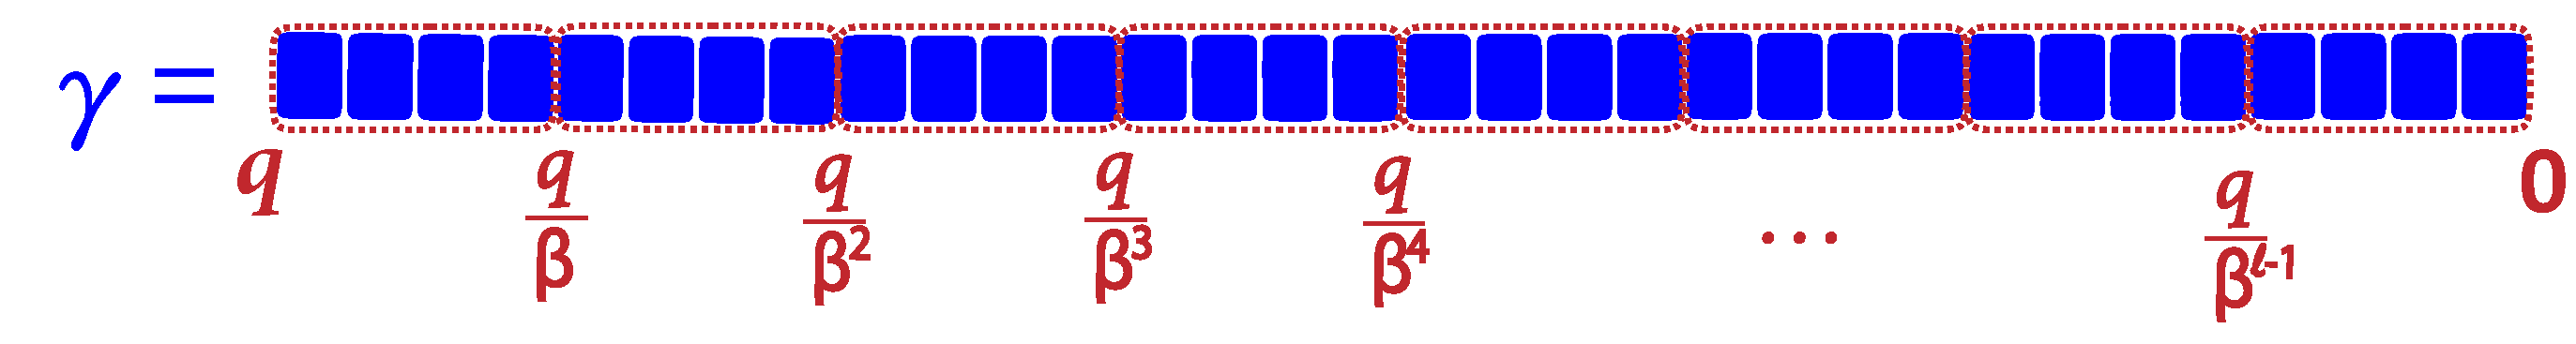
\includegraphics[width=0.8\linewidth]{figures/decomp.pdf}
  \caption{An illustration of number decomposition.}
  \label{fig:decomp}
\end{figure}

We define the decomposition of number $\gamma$ into base $\beta$ with level $\ell$ as follows:


$ $

$\textsf{Decomp}^{\beta, \ell}(\gamma) = (\gamma_1, \gamma_2, \text{ } \cdots , \text{ } \gamma_\ell)$.
 
$ $

Number decomposition is also called radix decomposition, where the base $\beta$ is called a radix. 


\subsubsection{Example}

Suppose we take $\gamma=13$ in $\mathbb{Z}_{16}$. Suppose we want to decompose 13 with the base $\beta = 2$ and level $\ell = 4$. Then, 13 is decomposed as follows:

$ $

$13 = 1 \cdot \dfrac{16}{2^1} + 1 \cdot \dfrac{16}{2^2} + 0 \cdot \dfrac{16}{2^3} + 1 \cdot \dfrac{16}{2^4}$

$ $

$\textsf{Decomp}^{2, 4}(13) = (1, 1, 0, 1)$


\subsection{Polynomial Decomposition}
\label{subsec:poly-decomp}

This time, suppose we have polynomial $f$ in the polynomial ring ${\mathbb{Z}_q[x] / (x^n + 1)}$. Therefore, each coefficient $c_i$ of $f$ is an integer modulo $q$. Polynomial decomposition expresses $f$ as a sum of multiple polynomials in base $\beta$ and level $\ell$ as follows:


\begin{tcolorbox}[title={\textbf{\tboxlabel{\ref*{subsec:poly-decomp}} Polynomial Decomposition}}]

Given $f\in \mathbb{Z}_q[x]/(x^n+1)$, fix $\beta\ge 2$ and $\ell\ge 1$ with $\beta^\ell\mid q$. We write

$ $

$f=\sum_{i=1}^{\ell} f_i\,\frac{q}{\beta^i}, \qquad f_i\in \mathbb{Z}_q[x]/(x^n+1)  $

$ $

where each $f_i$ is obtained by decomposing every coefficient of $f$ in base $\beta$. If $f=\sum_j c_j x^j$ with $c_j\in\mathbb{Z}_q$, then
$c_j=\sum_{i=1}^{\ell} c_{j,i}\, \frac{q}{\beta^i}$ with $c_{j,i}\in\{0,\ldots,\beta-1\}$,
and $f_i=\sum_j c_{j,i} x^j$.
We denote the decomposition of the polynomial $f$ into the base $\beta$ with the level $\ell$ as follows:

$ $

$\textsf{Decomp}^{\beta, \ell}(f) = (f_1, f_2, \text{ } \cdots , \text{ } f_\ell)$
 $ $
\end{tcolorbox}




\subsubsection{Example}

Suppose we have the following polynomial in the polynomial ring $\mathbb{Z}_{16}[x] / (x^4 + 1)$:

$ $

$f = 6x^3 + 3x^2 + 14x + 7 \in \mathbb{Z}_{16}[x] / (x^4 + 1)$

$ $

Suppose we want to decompose the above polynomial with base $\beta = 4$ and level $\ell = 2$. Then, each degree's coefficient of the polynomial $f$ is decomposed as follows:

$ $

${\bm{x}^{\bm{3}}}$: $6 = \color{blue}{1 \cdot \dfrac{16}{4^1}} \color{black}+ \color{red}{2 \cdot \dfrac{16}{4^2}}$

${\bm{x}^{\bm{2}}}$: $3 = \color{blue}{0 \cdot \dfrac{16}{4^1}} \color{black}+ \color{red}{3 \cdot \dfrac{16}{4^2}}$

${\bm{x}^{\bm{1}}}$: $14 = \color{blue}{3 \cdot \dfrac{16}{4^1}} \color{black}+ \color{red}{2 \cdot \dfrac{16}{4^2}}$

${\bm{x}^{\bm{0}}}$: $7 = \color{blue}{1 \cdot \dfrac{16}{4^1}} \color{black}+ \color{red}{3 \cdot \dfrac{16}{4^2}}$

$ $

The decomposed polynomial is as follows:

$f = 6x^3 + 3x^2 + 14x + 7 = \color{blue}{(1x^3 + 0x^2 + 3x + 1) \cdot \dfrac{16}{4^1}} \color{black}+ \color{red}{(2x^3 + 3x^2 + 2x + 3) \cdot \dfrac{16}{4^2}} \color{black}$

$ $

$\textsf{Decomp}^{4, 2}(6x^3 + 3x^2 + 14x + 7) = (1x^3 + 0x^2 + 3x + 1, 2x^3 + 3x^2 + 2x + 3)$

\subsubsection{Discussion}

Note that after decomposition, the original coefficients of the polynomial got reduced to smaller numbers. This characteristic is importantly used in homomorphic encryption's multiplication, for reducing the growth rate of the noise. Normally, the polynomial coefficients of ciphertexts are large because they are uniformly random numbers. Reducing such big constants is important to reduce the noise growth during homomorphic multiplication. We will discuss this more in detail in \autoref{subsec:tfhe-mult-cipher}.


\subsection{Approximate Decomposition}
\label{subsec:approx-decomp}

\begin{figure}[h!]
    \centering
  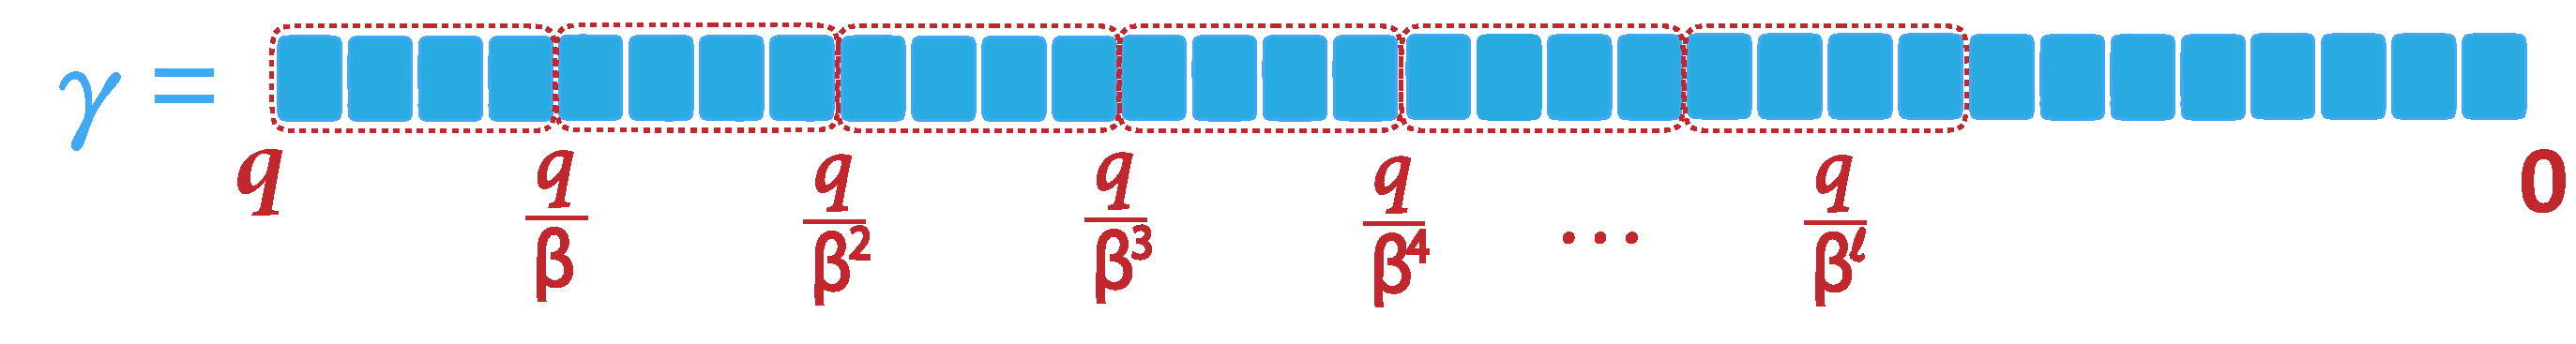
\includegraphics[width=0.7\linewidth]{figures/decomp3.pdf}
  \caption{An illustration of approximate decomposition}
  \label{fig:decomp3}
\end{figure}

If no level $\ell$ satisfies $\beta^\ell \mid q$, then some lower bits of $q$ must be discarded during decomposition, as shown in \autoref{fig:decomp3}. Such lower bits can be rounded to the nearest multiple of $\dfrac{q}{\beta^\ell}$ during decomposition. In such a case, the decomposition is an approximate decomposition. 
Formally, when $\beta^\ell\nmid q$ we can write
$$
\gamma=\sum_{i=1}^{\ell}\gamma_i\,\frac{q}{\beta^{i}}+\varepsilon,\qquad
\gamma_i\in\{0,\ldots,\beta-1\},\quad
|\varepsilon|\le \frac{q}{2\beta^{\ell}}
$$
(using nearest-integer rounding and identifying $\gamma$ with its integer representative). The polynomial case is analogous, coefficient-wise.



\subsection{Gadget Decomposition}
\label{subsec:gadget-decomposition}

Gadget decomposition is a generalized form of number decomposition (\autoref{subsec:number-decomp}). In number decomposition, a number $\gamma$ is decomposed as follows: 

$\gamma = \gamma_1 \dfrac{q}{\beta^1} + \gamma_2 \dfrac{q}{\beta^2} + \cdots + \gamma_\ell \dfrac{q}{\beta^\ell} $

$ $

In gadget decomposition, we decompose $\gamma$ as follows: 

$\gamma = \gamma_1 g_1 + \gamma_2 g_2 + \cdots + \gamma_\ell g_\ell $

$ $

We denote $\vec{g} = (g_1, g_2, \cdots, g_\ell)$ as a gadget vector, and $\textsf{Decomp}^{\vec{g}}(\gamma) = (\gamma_1, \gamma_2, \text{ } \cdots , \text{ } \gamma_\ell) $

$ $

Then, $\gamma = \langle \textsf{Decomp}^{\vec{g}}(\gamma), \vec{g} \rangle $

$ $

In the case of number decomposition (\autoref{subsec:number-decomp}), its gadget vector is $\vec{g} = \Bigg(\dfrac{q}{\beta}, \dfrac{q}{\beta^2}, \cdots, \dfrac{q}{\beta^\ell}\Bigg)$.




%\clearpage
%\input{scratch-real}

\end{document}


%https://www.youtube.com/watch?v=vYKdh5oQ4Zw
